\documentclass[12pt, letterpaper]{article}
\usepackage{graphicx} % Required for inserting images
\usepackage[vietnamese]{babel}
\usepackage[a4paper, left=3cm, right=2cm, top=2.5cm, bottom=2.5cm]{geometry}
\usepackage{mathptmx} %font time new roman
\usepackage{float} %set vị trí chèn ảnh
\usepackage{tikz} %tạo khung bìa
\usetikzlibrary{calc} %thư viện tikz
\usepackage{indentfirst} % Thụt đầu dòng
\renewcommand{\baselinestretch}{1.2} % Giãn dòng 1.2
\setlength{\parskip}{6pt} % Khoảng cách sau đoạn
\usepackage{titlesec} % Thư viện để set up các kiểu chữ
\usepackage{xcolor}    % để dùng màu
\usepackage{fancyvrb}   % để chỉnh màu cho verbatim
\DefineVerbatimEnvironment{verbatim}{Verbatim}
{formatcom=\color{purple}} % đổi chữ verbatim thành màu xanh lá
\setlength{\parindent}{0pt}
\titlespacing*{\section}{0pt}{0pt}{30pt} % Heading 1
\titleformat*{\section}{\fontsize{16pt}{0pt}\selectfont\bfseries}
\titlespacing*{\subsection}{0pt}{10pt}{0pt} % Heading 2
\titleformat*{\subsection}{\fontsize{14pt}{0pt}\selectfont\bfseries}
\titlespacing*{\subsubsection}{0pt}{10pt}{0pt} % Heading 3
\titleformat*{\subsubsection}{\fontsize{13pt}{0pt}\selectfont\bfseries\itshape}
\titlespacing*{\paragraph}{0pt}{10pt}{0pt} % Heading 4
\titleformat*{\paragraph}{\fontsize{13pt}{0pt}\selectfont\itshape}
\setcounter{secnumdepth}{4}
\usepackage[colorlinks=true, urlcolor=blue, linkcolor=black]{hyperref}
\usepackage{enumitem} % dùng để kiểm soát đẹp hơn
\renewcommand{\labelitemii}{\small$\blacksquare$}
\begin{document}
\begin{titlepage}
    \begin{tikzpicture}[overlay, remember picture]
    % Vẽ khung lớn
    \draw [line width=3pt]
        ($ (current page.north west) + (3.0cm,-2.0cm) $)
        rectangle
        ($ (current page.south east) + (-2.0cm,2.5cm) $);
    
    % Vẽ khung nhỏ
    \draw [line width=0.5pt]
        ($ (current page.north west) + (3.1cm,-2.1cm) $)
        rectangle
        ($ (current page.south east) + (-2.1cm,2.6cm) $);
    \end{tikzpicture}
    \begin{center}
        \textbf{\fontsize{16pt}{0pt}\selectfont HỌC VIỆN CÔNG NGHỆ BƯU CHÍNH VIỄN THÔNG} \\
        \vspace{10pt}
        \begin{figure}[h]
            \centering
            
\includegraphics[width=0.5\linewidth]{img/logo.png}
        \end{figure}
         \textbf{\fontsize{26pt}{0pt}\selectfont BÀI TẬP LỚN} \\
         \vspace{10pt}
         \textbf{\fontsize{26pt}{0pt}\selectfont MÔN: LẬP TRÌNH PYTHON} \\
         \vspace{2cm}
    \end{center}
    \begin{table}[H]
         \centering
         \begin{tabular}{c c}
           \textbf{\fontsize{14pt}{0pt}\selectfont HỌ TÊN:}   &  \fontsize{14pt}{0pt}\selectfont Đỗ Tiến Thành \vspace{6pt} \\
           \textbf{\fontsize{14pt}{0pt}\selectfont MÃ SV:}   &  \fontsize{14pt}{0pt}\selectfont B23DCDT239 \vspace{6pt} \\
           \textbf{\fontsize{14pt}{0pt}\selectfont LỚP:}   &  \fontsize{14pt}{0pt}\selectfont D23CQCE04-B \\
         \end{tabular}
     \end{table}
\end{titlepage}
\cleardoublepage
\addtocontents{toc}{\protect\thispagestyle{empty}}
\tableofcontents
\thispagestyle{empty}

\cleardoublepage

% ĐỀ BÀI
\pagenumbering{arabic}
\section{YÊU CẦU ĐỀ BÀI}
\addcontentsline{toc}{section}{\numberline {} YÊU CẦU ĐỀ BÀI}
\setcounter{section}{0}
\subsection{Problem 1}
Write a Python program to collect footballer player statistical data with the following
requirements:
\begin{itemize}
    \item Collect statistical data [*] for all players who have played more than 90 minutes in the
2024-2025 English Premier League season.
    \item Data source: \url{https://fbref.com/en/}
    \item Save the result to a file named 'results.csv', where the result table has the following
structure:
    \begin{itemize}[label=$\circ$]
        \item Each column corresponds to a statistic.
        \item Players are sorted alphabetically by their first name.
        \item Any statistic that is unavailable or inapplicable should be marked as "N/a".
    \end{itemize}
    \item The required statistics are:
    \begin{itemize}[label=$\circ$]
        \item \textbf{Nation}
        \item \textbf{Team}
        \item \textbf{Position}
        \item \textbf{Age}
        \item \textbf{Playing Time}: matches played, starts, minutes
        \item \textbf{Performance}:  expected goals (xG), expedted Assist Goals (xAG)
        \item \textbf{Progression}: PrgC, PrgP, PrgR
        \item \textbf{Per 90 minutes}: Gls, Ast, xG, xGA
        \item \textbf{Goalkeeping}:
        \begin{itemize}
            \item Performance: goals against per 90mins (GA90), Save\%, CS\%
            \item Penalty Kicks: penalty kicks Save\%
        \end{itemize}
        \item \textbf{Shooting}:
        \begin{itemize}
            \item Standard: shoots on target percentage (SoT\%), Shoot on Target per 90min
(SoT/90), goals/shot (G/sh), average shoot distance (Dist)
        \end{itemize}
        \item \textbf{Passing}:
        \begin{itemize}
            \item Total: passes completed (Cmp),Pass completion (Cmp\%), progressive
passing distance (TotDist)
            \item Short: Pass completion (Cmp\%),
            \item Medium: Pass completion (Cmp\%),
            \item Long: Pass completion (Cmp\%),
            \item Expected: key passes (KP), pass into final third (1/3), pass into penalty
area (PPA), CrsPA, PrgP
        \end{itemize}
        \item \textbf{Goal and Shot Creation}:
        \begin{itemize}
            \item SCA: SCA, SCA90
            \item GCA: GCA, GCA90
        \end{itemize}
        \item \textbf{Defensive Actions}:
        \begin{itemize}
            \item Tackles: Tkl, TklW
            \item Challenges: Att, Lost
            \item Blocks: Blocks, Sh, Pass, Int
        \end{itemize}
        \item \textbf{Possession}:
        \begin{itemize}
            \item Touches: Touches, Def Pen, Def 3rd, Mid 3rd, Att 3rd, Att Pen
            \item Take-Ons: Att, Succ\%, Tkld\%
            \item Carries: Carries, ProDist, ProgC, 1/3, CPA, Mis, Dis
            \item Receiving: Rec, PrgR
        \end{itemize}
        \item \textbf{Miscellaneous Stats}:
        \begin{itemize}
            \item Performance: Fls, Fld, Off, Crs, Recov
            \item Aerial Duels: Won, Lost, Won%
        \end{itemize}
    \end{itemize}
\end{itemize}
\subsection{Problem 2}
\begin{itemize}
    \item Identify the top 3 players with the highest and lowest scores for each statistic. Save result to a file name ‘top\_3.txt’
    \item Find the median for each statistic. Calculate the mean and standard deviation for each
statistic across all players and for each team. Save the results to a file named 'results2.csv'
with the following format:
    \begin{table}[H]
        \centering
        \begin{tabular}{|c|c|c|c|c|c|c|}
            \hline
              & Median of Attribute 1 & Mean of Attribute 1 & Std of Attribute 1 & \ldots & \ldots & \ldots \\
            \hline
            0 & all & & & & & \\
            \hline
            1 & Team 1 & & & & & \\
            \hline
            \ldots & \ldots & \ldots & \ldots & \ldots & \ldots & \ldots \\
            \hline
            n & Team n & & & & & \\
            \hline
        \end{tabular}
    \end{table}
    \item Plot a histogram showing the distribution of each statistic for all players in the league and each team.
    \item Identify the team with the highest scores for each statistic. Based on your analysis, which team do you think is performing the best in the 2024-2025 Premier League season?
\end{itemize}
\subsection{Problem 3}
\begin{itemize}
    \item Use the K-means algorithm to classify players into groups based on their statistics.
    \item How many groups should the players be classified into? Why? Provide your comments
    on the results.
    \item Use PCA to reduce the data dimensions to 2, then plot a 2D cluster of the data points.
\end{itemize}
\subsection{Problem 4}
\begin{itemize}
    \item Collect player transfer values for the 2024-2025 season from \\
    \url{https://www.footballtransfers.com.} Note that only collect for the players whose playing
    time is greater than 900 minutes
    \item Propose a method for estimating player values. How do you select feature and model?
\end{itemize}
\cleardoublepage

\section{PHÂN TÍCH CÂU 1}
\addcontentsline{toc}{section}{\numberline {} PHÂN TÍCH CÂU 1}
\setcounter{section}{1}
* \textbf{Truy cập link github để có thể xem code tốt nhất:}  \url{https://github.com/DoTienThanh325/Big_exercise/tree/main/Problem%201}
\subsection{Ý tưởng làm bài}
Truy cập từng url có số liệu của từng đội bóng một lấy các số liệu theo yêu cầu của đề bài. Mỗi url lấy số liệu ở 8 bảng: 
\begin{itemize}
    \item \textbf{Standard Stats} 
    \item \textbf{Goalkeeping}
    \item \textbf{Shooting}
    \item \textbf{Passing}
    \item \textbf{Goal and Shot Creation}
    \item \textbf{Defensive Actions}
    \item \textbf{Possession}
    \item \textbf{Miscellaneous Stats}
\end{itemize}
Sau đó gộp các bảng của một đội bóng lại thành một chuyển các dữ liệu kiểu null -> 'N/a'. Làm tương tự với tất cả các đội bóng rồi ghép các bảng dữ liệu lại làm một.
\subsection{Phân tích code câu 1}
\vspace{6pt}
\subsubsection{Hàm đặt lại tên cột}
    \begin{figure}[h]
        \centering
        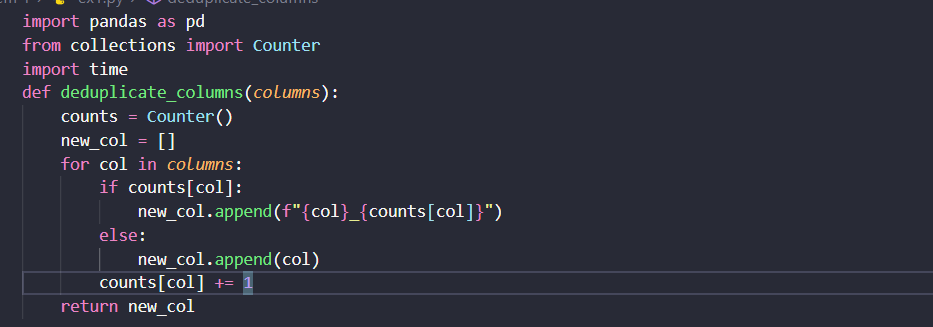
\includegraphics[width=1\textwidth]{img/ham_rename_col.png}
    \end{figure}
    - Sử dụng thư viện collections để đếm số lần xuất hiện của cột.
    - Duyệt qua tất cả các cột có trong dataframe kiểm tra số lần xuất hiện thông qua. counts[col]
    \begin{itemize}
        \item Nếu cột có counts[col] == 0 tức là lần đầu được duyệt -> đẩy vào list new\_col.
        \item Nếu cột có counts[col] != 0 -> đưa vào new\_col với tên mới là \textbf{tên côt + số lần xuất hiện}.
    \end{itemize}
    
\subsubsection{Hàm cài đặt Dataframe}
    - Tạo hàm crawl\_data\_table chuyền vào ba tham số là df(dữ liệu dataframe), list(các cột dữ liệu đề bài yêu cầu), club(tên câu lạc bộ).\\
    \begin{figure}[H]
        \centering
        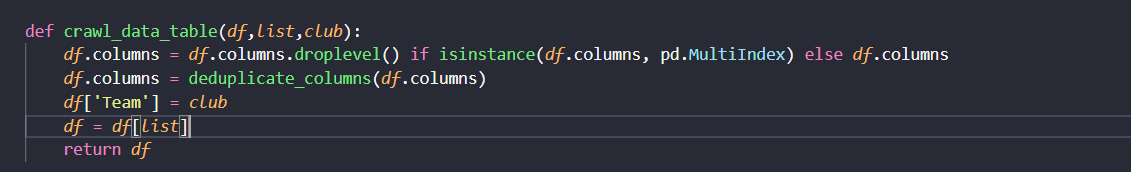
\includegraphics[width=1\textwidth]{img/set_df.png}
    \end{figure}
    - \textbf{\textit{df.columns = df.columns.droplevel() if isinstance(df.columns, pd.MultiIndex) else df.columns}}: câu lệnh xóa bỏ kiểu multiindex của col.
    \begin{itemize}
        \item Kiểm tra xem hàng các cột có phải kiểu multiindex không: \textbf{\textit{isinstance(df.columns, pd.MultiIndex)}}.
        \item Nếu df.columns là kiểu multiindex thì xóa bỏ  \textbf{\textit{df.columns.droplevel()}} không thì giữ nguyên.
    \end{itemize}
    - \textbf{\textit{df.columns = deduplicate\_columns(df.columns)}}: Gọi hàm deduplicate\_columns để đạt lại tên các cột do có các cột bị trùng tên.\\
    - \textbf{\textit{df['Team'] = club}}: Thêm cột Team với giá trị là club.\\
    - \textbf{\textit{df = df[list]}}: Cài đặt lại dataframe lấy các giá trị theo đề bài.

\subsubsection{Hàm tạo Dataframe}
    - Cài đặt hàm trả về một dataframe\\
    \begin{figure}[H]
        \centering
        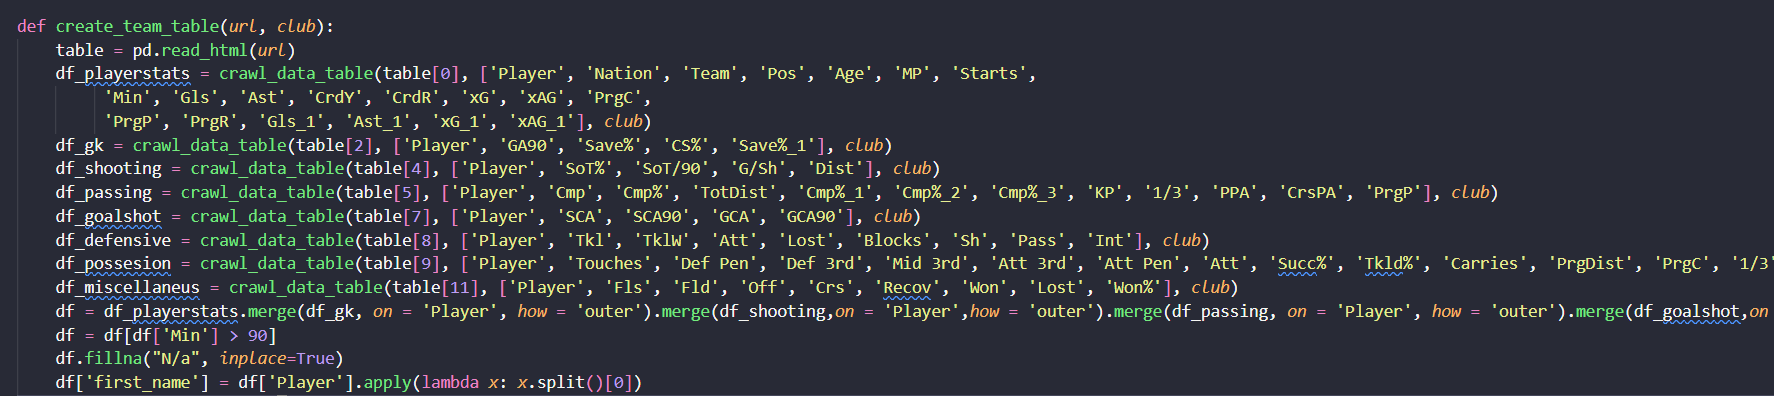
\includegraphics[width=1\textwidth, height=6cm]{img/tao_bang.png}
    \end{figure}
    - Sử dụng hàm \textbf{read\_html()} trong thư viện pandas để đọc các bảng dữ liệu có trong url.\\
    - Khởi tạo các dataframe \textbf{\textit{df\_playerstats, df\_gk, df\_shooting, df\_passing, df\_goalshot, df\_defensive, df\_possesion, df\_miscellaneus}} bàng hàm \textbf{\textit{crawl\_data\_table}} với vị trí bảng tương ứng trong url và các giá trị đề bài yêu cầu cùng tên club.\\
    - Khởi tạo dataframe \textbf{df} là dataframe tổng của các dataframe trên bằng cách \textbf{merge} tất cả các dataframe trên lại dựa vào thuộc tính \textbf{on = 'Player'} (merge các dataframe dựa vào tên cầu thủ) và cách thức \textbf{how = 'outer'} (thêm các giá trị mà dataframe trước không có).\\
    - \textbf{df = df[df['Min] > 90]}: Chỉ lấy các cầu thủ có thời gian trên 90 phút.\\
    - \textbf{df.fillna("N/a", inplace=True)}: Thay thế tất cả các giá trị null bằng 'N/a'.\\
    \begin{figure}[H]
        \centering
        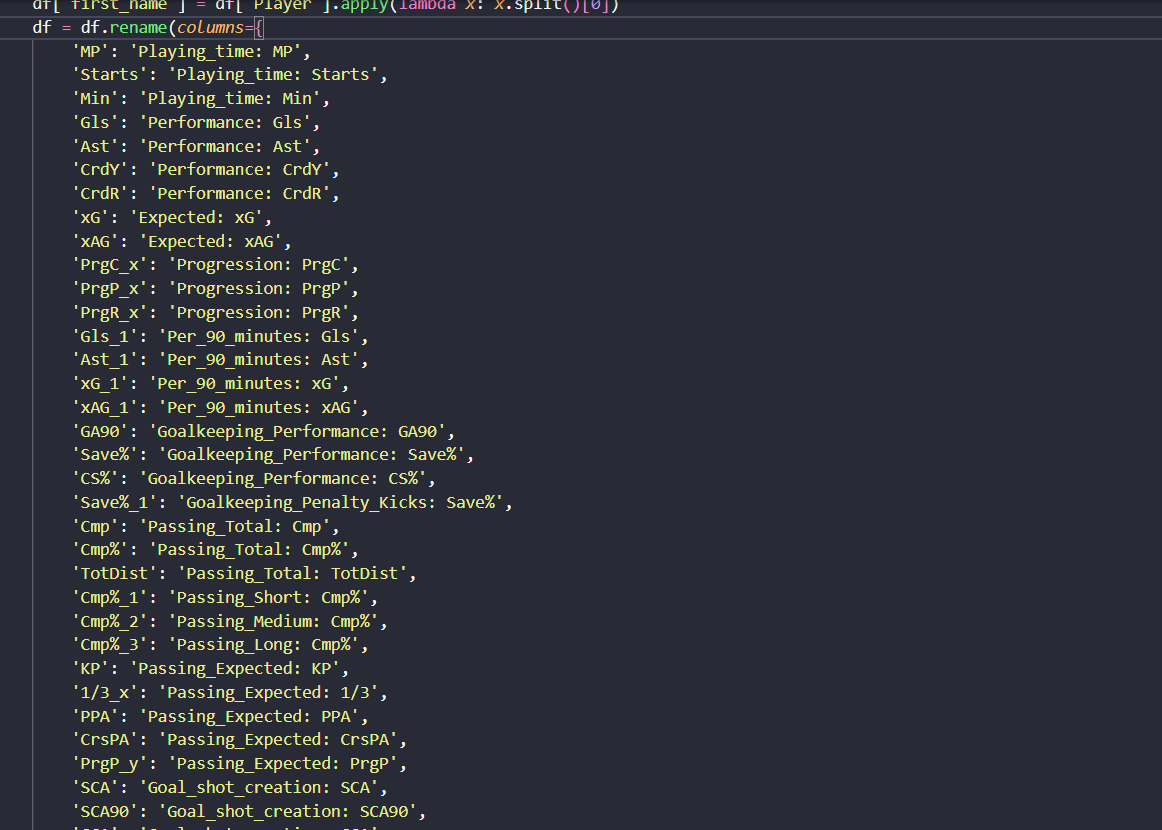
\includegraphics[width=1\linewidth, height=15cm]{img/rename.png}
    \end{figure}
    - Sử dụng hàm \textbf{rename} có sẵn trong thư viện pandas để cài đặt lại tên các cột.\\
    - Tên các cột bằng \textbf{Tên các nhóm chỉ số + tên chỉ số}.\\
    VD: chỉ số \textbf{Gls} trong nhóm chỉ số \textbf{Performance} -> \textbf{Performance: Gls}\\
    - Cuối cùng hàm trả về dataframe hoàn chỉnh.\\

\subsubsection{Viết chương trình trong hàm main}
    \begin{figure}[H]
        \centering
        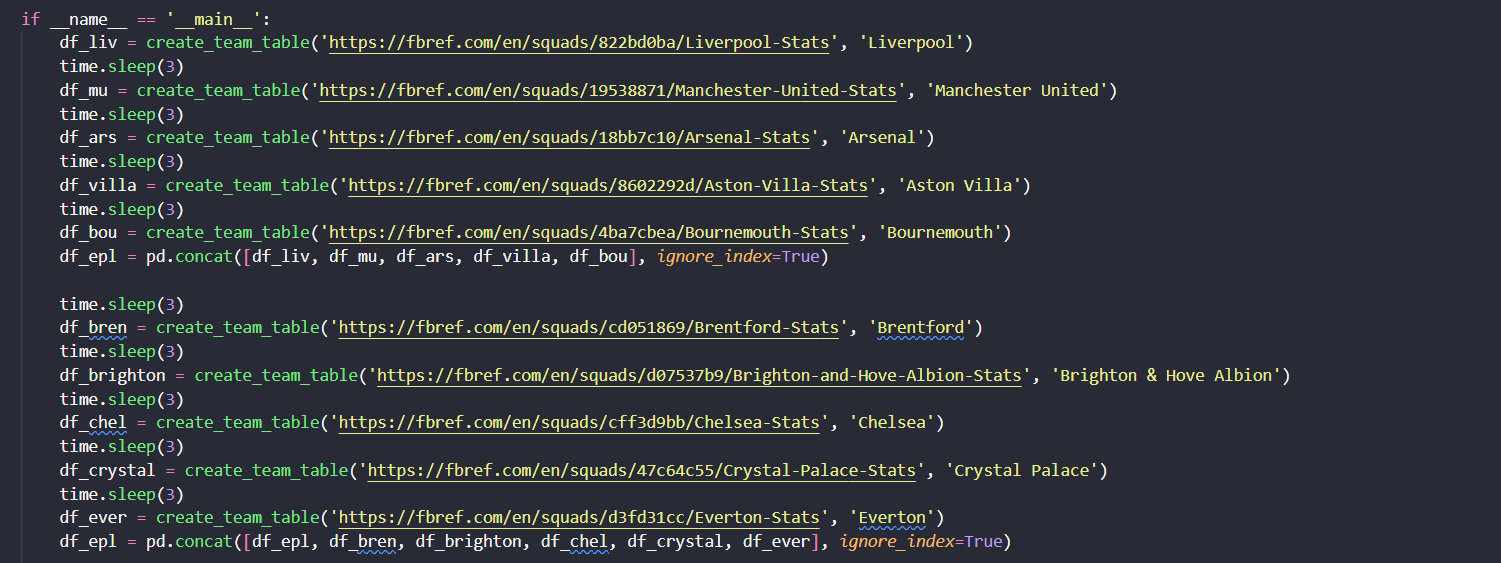
\includegraphics[width=1\linewidth]{img/collect_10_team_first.png}
    \end{figure}
    \begin{figure}[H]
        \centering
        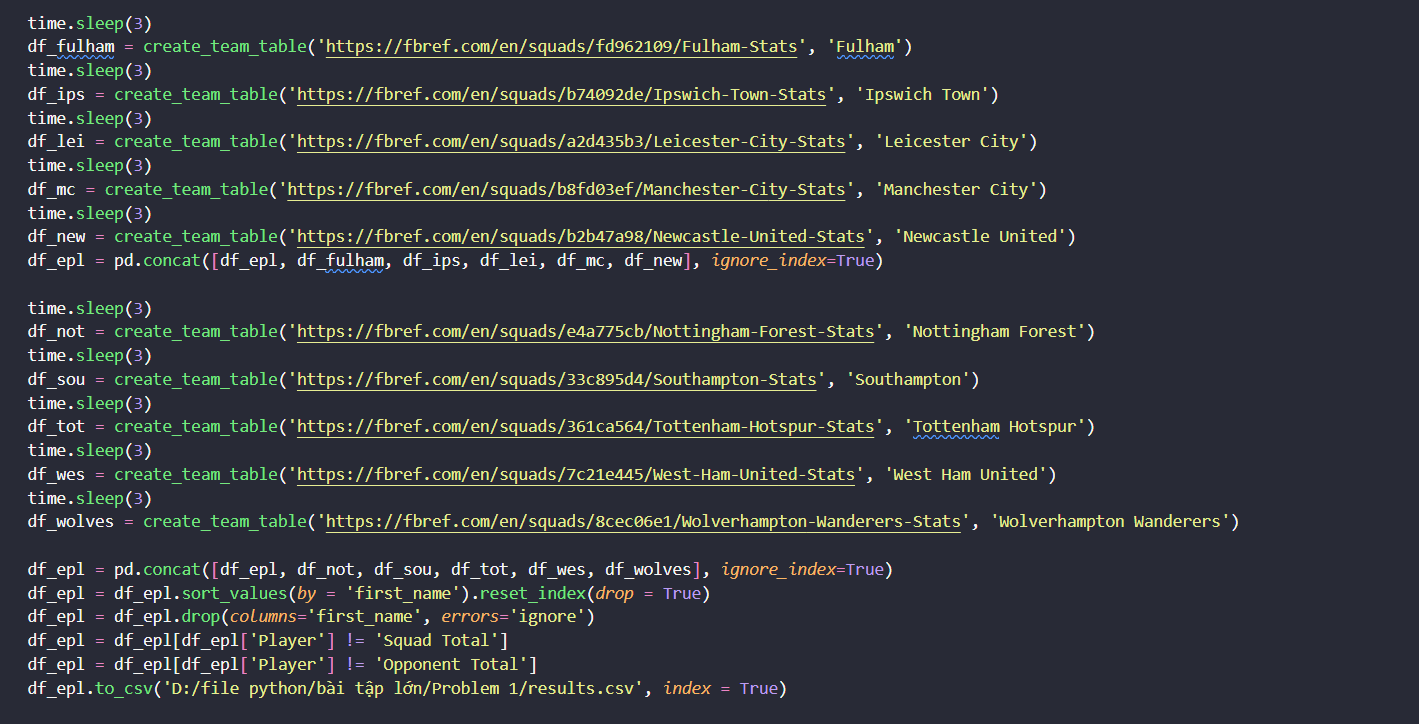
\includegraphics[width=1\linewidth]{img/collect_10_second.png}
    \end{figure}
    - Viết chương trình trong hàm main.\\
    - Sử dụng hàm \textbf{create\_team\_table} để tạo dataframe cho từng đội bóng.\\
    - Giữa mỗi lần lấy dữ liệu của đội bóng thêm \textbf{time.sleep(3)} để tránh bị web chặn.\\
    - Khởi tạo \textbf{\textit{df\_epl}} bằng gộp các dataframe đội bóng bằng hàm \textbf{concat} trong thư viện pandas với \textbf{ignore\_index=True} (khởi tạo lại index cho dataframe sau khi gộp).\\
    - Chia nhỏ lần gửi request (5 đội bóng liên tiếp xong gộp vào với \textbf{df\_epl} luôn để tránh bị web chặn request).\\
    - Sau khi có dữ liệu của tất cả các cầu thủ trong dataframe \textbf{df\_epl} ta thực hiện sắp xếp theo \textbf{first\_name} có reset index sau khi sắp xếp: \textbf{df\_epl = df\_epl.sort\_values(by = 'first\_name')\\.reset\_index(drop = True)}.\\
    - Loại bỏ cột \textbf{first\_name} và các hàng có 'Player' = 'Squad Total' và 'Opponent Total':
    \begin{itemize}
        \item \textbf{df\_epl = df\_epl.drop(columns='first\_name', errors='ignore')}
        \item \textbf{df\_epl = df\_epl[df\_epl['Player'] != 'Squad Total']}
        \item \textbf{df\_epl = df\_epl[df\_epl['Player'] != 'Opponent Total']}
    \end{itemize}
    - Cuối cùng lưu kết quả dataframe hoàn chỉnh vào file 'results.csv' bằng câu lệnh: \\ 
    \textbf{df\_epl.to\_csv('D:/file python/bài tập lớn/Problem 1/results.csv', index = True)}

\cleardoublepage

\section{PHÂN TÍCH CÂU 2}
\addcontentsline{toc}{section}{\numberline {} PHÂN TÍCH CÂU 2}
\setcounter{section}{2}
* \textbf{Truy cập link github để có thể xem code tốt nhất:}  \url{https://github.com/DoTienThanh325/Big_exercise/tree/main/Problem%202}
\subsection{Câu 2 ý 1}
\subsubsection{Ý tưởng làm bài}
Lấy dữ liệu từ bài 1 đưa vào một dataframe lọc ra các cột chỉ số dữ liệu dưới dạng number. Duyệt qua các cột mỗi cột sắp xếp lại theo thứ tự giảm dần của chỉ số lấy ra ba cầu thủ đầu lưu vào file theo yêu cầu đề bài sau đó lại sắp xếp theo thứ tự tăng dần của các chỉ số của cột đó và lấy ba cầu thủ đầu để đưa vào file
\subsubsection{Phân tích code câu 2 ý 1}
    \begin{figure}[H]
        \centering
        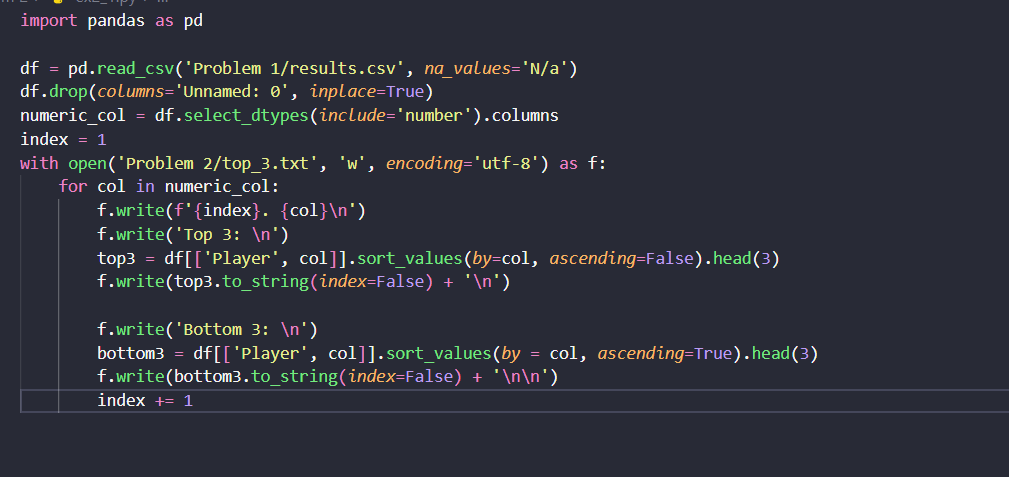
\includegraphics[width=1\linewidth]{img/2_1.png}
    \end{figure}
    - Lấy dữ liệu câu 1 thu được đưa vào dataframe \textbf{df} chuyển tất cả các chuỗi 'N/a' về dạng na bằng câu lệnh: \textbf{df = pd.read\_csv('Problem 1/results.csv', na\_values='N/a')}.\\
    - Loại bỏ cột 'Unnamed: 0' (Là cột index lưu từ câu 1): \textbf{df.drop(columns='Unnamed: 0', inplace=True)}.\\
    - Lấy ra list các cột có dữ liệu dạng số lưu vào \textbf{numeric\_col}: \\ \textbf{numeric\_col = df.select\_dtypes(include='number').columns}
    - Khởi tạo biến index bằng 1 để đánh dấu index các cột chỉ số.\\
    - Mở file để lưu dữ liệu phân tích vào:\\ \textbf{with open('Problem 2/top\_3.txt', 'w', encoding='utf-8') as f:}. \\
    - Dùng vòng \textbf{for} duyệt qua từng cột một, tại mỗi cột:
    \begin{itemize}
        \item Tìm ra ba cầu thủ có chỉ số cao nhất bằng cách sắp xếp dựa vào chỉ số của cột theo chiều giảm dần và đưa vào file:
        \begin{figure}[H]
            \centering
            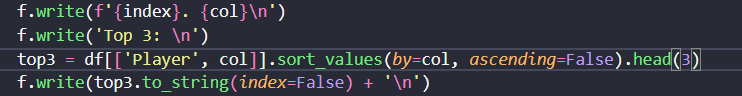
\includegraphics[width=1\linewidth]{img/top3.png}
        \end{figure}
        \item Tìm ra ba cầu thủ có chỉ số thấp nhất bằng cách sắp xếp dựa vào chỉ số của cột theo chiều tăng dần và đưa vào file:
        \begin{figure}[H]
            \centering
            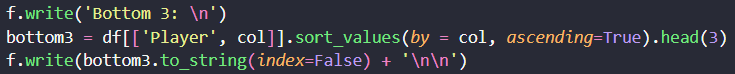
\includegraphics[width=1\linewidth]{img/bottom3.png}
        \end{figure}
    \end{itemize}
    - Sau cột ta lại tăng biến index lên một đơn vị.\\
\subsection{Câu 2 ý 2}
\subsubsection{Ý tưởng làm bài}
Lấy dữ liệu từ bài 1 đưa vào một dataframe lọc ra các cột chỉ số dữ liệu dưới dạng number. Tạo dictionary all\_team để lưu trữ dữ liệu của toàn bộ các đội bóng và có 'Team': 'all' duyệt qua các cột dữ liệu bên trên tính median, mean, std của từng cột và đưa vào dictionary với keys phù hợp sau đó đấy dictionary đó vào một list tổng. Với từng câu lạc bộ ta lấy tất cả cầu thủ thuộc đội bóng đưa vào một dataframe và làm tương tự như toàn giải đấu sau đó cũng đưa vào list tổng. Cuối cùng chuyển list tổng sang dạng dataframe và đấy vào file csv.
\subsubsection{Phân tích code câu 2 ý 2}
    \begin{figure}[H]
        \centering
        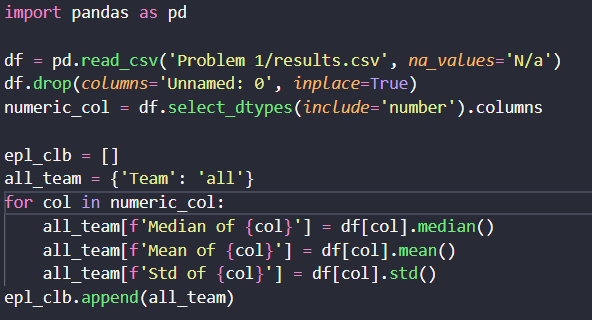
\includegraphics[width=1\linewidth]{img/2_2-1.png}
    \end{figure}
    - Lấy dữ liệu của file csv và chỉnh sửa giống ý 1.\\
    - Khởi tạo một list rỗng: \textbf{epl\_clb = []}
    - Tạo một dictionary có 1 keys là \textbf{Team} và values là \textbf{all}: \textbf{all\_team = \{'Team': 'all'\}}.\\
    - Duyệt qua từng cột của \textbf{numeric\_col}, mỗi cột tạo key và value tương ứng cho dictionary \textbf{all\_team}: \begin{verbatim}
        all_team[f'Median of {col}'] = df[col].median()
        all_team[f'Mean of {col}'] = df[col].mean()
        all_team[f'Std of {col}'] = df[col].std()
    \end{verbatim}
    - Thêm dictionary all\_team vào list epl\_clb: \textbf{epl\_clb.append(all\_team)}
    \begin{figure}[H]
        \centering
        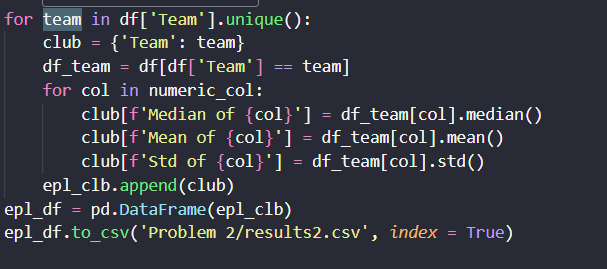
\includegraphics[width=1\linewidth]{img/2_2-2.png}
    \end{figure}
    - \textbf{for team in df['Team'].unique():}: Duyệt qua từng câu lạc bộ một.
    \begin{itemize}
        \item Mỗi câu lạc bộ tạo một dictionary là \textbf{club} với cặp key value đầu là \textbf{'Team': team} và tạo ra một dataframe lưu trữ toàn bộ cầu thủ của câu lạc bộ đó:
        \begin{verbatim}
            club = {'Team': team}
            df_team = df[df['Team'] == team]
        \end{verbatim}
        \item Duyệt qua từng cột và làm tương tự như toàn giải
        \begin{verbatim}
            for col in numeric_col:
                club[f'Median of {col}'] = df_team[col].median()
                club[f'Mean of {col}'] = df_team[col].mean()
                club[f'Std of {col}'] = df_team[col].std()
            epl_clb.append(club)
        \end{verbatim}
    \end{itemize}
    - Cuối cùng đưa list về dạng dataframe và lưu vào file csv:
    \begin{verbatim}
        epl_df = pd.DataFrame(epl_clb)
        epl_df.to_csv('Problem 2/results2.csv', index = True)
    \end{verbatim}

\subsection{Câu 2 ý 3}
\subsubsection{Ý tưởng làm bài}
Lấy những dữ liệu cột dưới dạng số sau đó dùng thư viện matplotlib để vẽ. Dùng subplots để có thể vẽ nhiều biểu đồ cùng một lúc
\subsubsection{Phân tích code câu 2 ý 3}
    \begin{figure}[H]
        \centering
        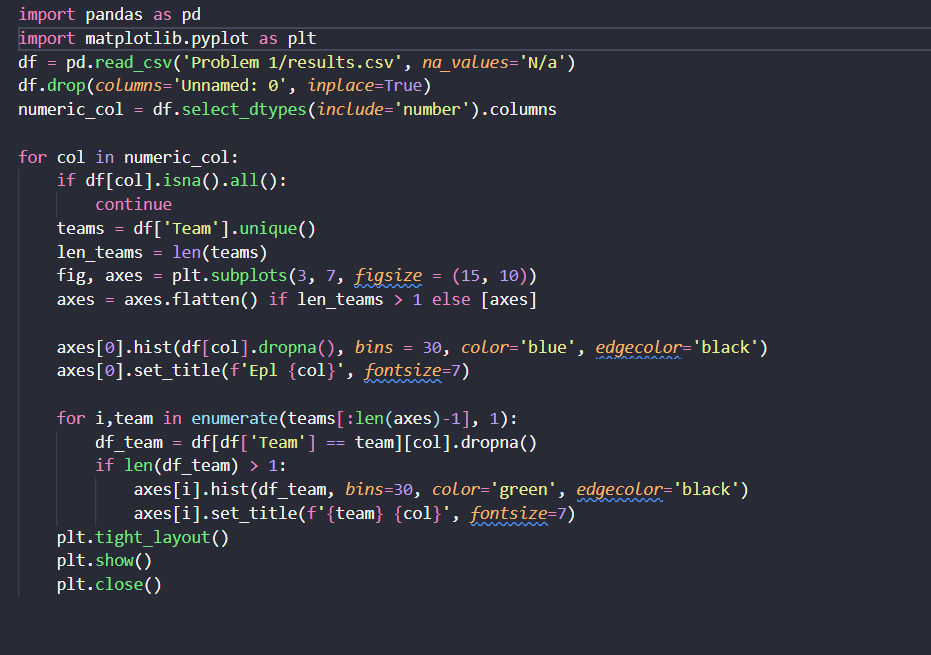
\includegraphics[width=1\linewidth]{img/2_3.png}
    \end{figure}
    - Đọc và xử lý dữ liệu như hai ý trên của câu 2.\\
    - Duyệt qua các cột:
    \begin{itemize}
        \item Nếu cột toàn \textbf{na} ta sẽ chuyển sang cột khác:
        \begin{verbatim}
        for col in numeric_col:
            if df[col].isna().all(): continue
        \end{verbatim}
        \item \textbf{teams = df['Team'].unique()}: Lấy danh sách các đội bóng không trùng trong cột 'Team'.
        \item \textbf{fig, axes = plt.subplots(3, 7, figsize=(15, 10))}: Tạo ra một figure với 3 hàng, 7 cột ô (tức là 21 ô) để vẽ các biểu đồ nhỏ (subplots).
        \item \textbf{axes = axes.flatten() if len\_teams > 1 else [axes]}: Vì axes ban đầu là một mảng 2D (3x7), nên bẻ phẳng thành 1D list cho dễ lặp. Còn nếu chỉ có 1 team thì axes không phải mảng, nên cho vào list để tránh lỗi.
        \item \textbf{axes[0].hist(df[col].dropna(), bins = 30, color='blue', edgecolor='black')}: Vẽ biểu đồ tần suất của cả giải trên subplot đầu tiên \textbf{axes[0]}. \textbf{dropna()} để loại bỏ giá trị NaN (trống) trước khi vẽ. \textbf{bins=30}: chia thành 30 cột nhỏ.  \textbf{color='blue'}: màu bên trong cột.  \textbf{edgecolor='black'}: viền cột màu đen.
        \item \textbf{axes[0].set\_title(f'Epl {col}', fontsize=7)}: Gắn tựa đề cho subplot. . \textbf{fontsize=7}: cỡ chữ cho tiêu đề.
        \item \textbf{enumerate(teams[:len(axes)-1], 1)}: Bắt đầu từ i = 1 (vì axes[0] đã dùng để vẽ EPL tổng). teams[:len(axes)-1]: tránh bị lỗi nếu số đội > số subplot.
        \item \textbf{df\_team = df[df['Team'] == team][col].dropna()}: Lọc ra dữ liệu cột col của từng đội. \textbf{dropna()} để không vẽ các giá trị thiếu.
        \item Đoạn code:
    \begin{verbatim}
    if len(df_team) > 1:
        axes[i].hist(df_team, bins=30, color='green', edgecolor='black')
        axes[i].set_title(f'{team} {col}', fontsize=7)
    \end{verbatim}
        kiểm tra \textbf{len(df\_team)} > 1 không để đảm bảo không lỗi. Hai câu sau giống như cách vễ biểu đồ tổng khác ở màu của cột là màu xanh lá cây.
        \item \textbf{plt.tight\_layout()}: Loại bỏ các biểu đồ rỗng.
        \item \textbf{plt.show()}: Hiển thị các biểu đồ khi run code.
        \item \textbf{plt.close()}: Xóa figure đã vẽ xong ra khỏi bộ nhớ.
    \end{itemize}
\subsection{Câu 2 ý 4} 
\subsubsection{Ý tưởng làm bài}
Tính trung bình cộng tất cả các chỉ số dưới dạng số liệu chọn ra đội đứng đầu ở nhiều nhất các chỉ số là đội có màn trình diễn tốt nhất.
\subsubsection{Phân tích code câu 2 ý 4}
\begin{figure}[H]
    \centering
    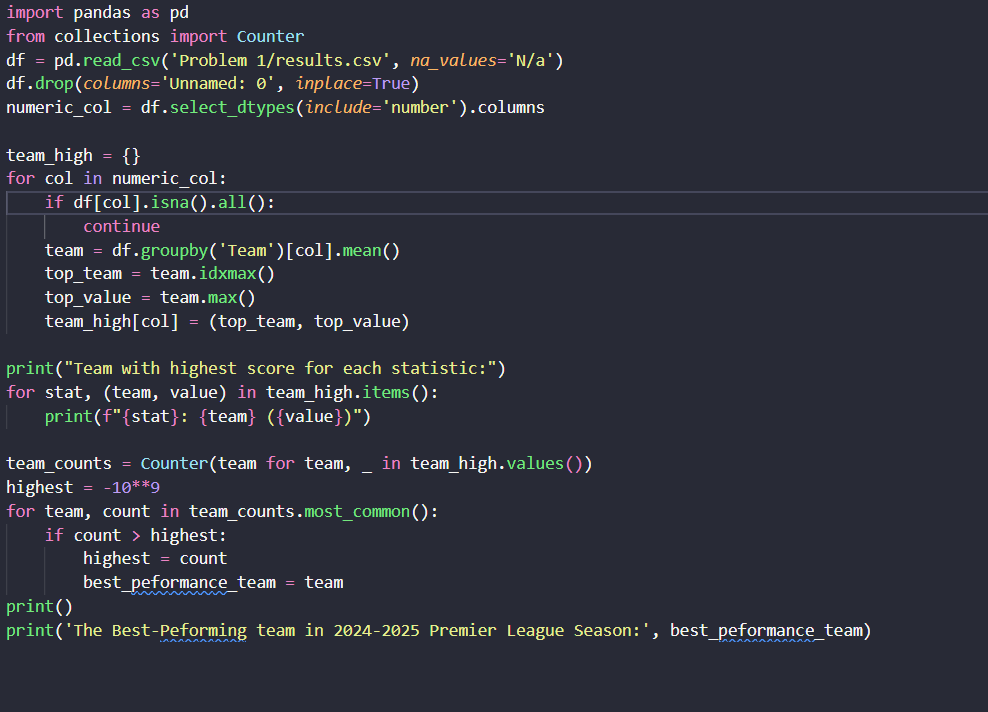
\includegraphics[width=1\linewidth]{img/2-4.png}
\end{figure}
- Xử lý dữ liệu như các ý trên của câu 2.\\
- \textbf{for col in numeric\_col:}: Duyệt qua các cột giá trị.\\
- \textbf{if df[col].isna().all(): continue}: Cột nào toàn giá trị NaN thì chuyển qua cột khác.\\
- \textbf{team = df.groupby('Team')[col].mean()}: Sử dụng hàm \textbf{groupby()} và hàm \textbf{mean()} để tính trung bình cộng các chỉ số của từng đội.\\
- \textbf{top\_team = team.idxmax()}: Dùng hàm \textbf{idxmax()} tìm ra đội có chỉ số trung bình cộng cao nhất.\\
- \textbf{top\_value = team.max()}: Dùng hàm \textbf{max()} tìm ra chỉ số cao nhất.\\
- \textbf{team\_high[col] = (top\_team, top\_value)}: Dùng dictionary để lưu trữ với key là tên cột và value là một tuple gồm hai giá trị \textbf{top\_team} và \textbf{top\_value}.\\
- Đoạn code:
    \begin{verbatim}
    print("Team with highest score for each statistic:")
    for stat, (team, value) in team_high.items():
        print(f"{stat}: {team} ({value})")
    \end{verbatim}
    \begin{itemize}
        \item Dùng để in các đội đứng đầu tại chỉ số và chỉ số đó
    \end{itemize}
- \textbf{team\_counts = Counter(team for team, \_ in team\_high.values())}: Tạo mảng đếm để đếm xem mỗi đội đứng đầu mỗi chỉ số bao lần, đội đứng đầu nhiều nhất là đội có best-peforming.\\
- Đoạn code:
    \begin{verbatim}
    highest = -10**9
    for team, count in team_counts.most_common():
        if count > highest:
            highest = count
            best_peformance_team = team 
    \end{verbatim}
    \begin{itemize}
        \item Đoạn code này dùng để tìm đội có số lần đứng đầu và gán cho biến \textbf{best\_peformance\_team} là đội bóng có số lần đứng đầu nhiều nhất.
    \end{itemize}

\cleardoublepage
\section{PHÂN TÍCH CÂU 3}
\addcontentsline{toc}{section}{\numberline {} PHÂN TÍCH CÂU 3}
\setcounter{section}{3}
* \textbf{Truy cập link github để có thể xem code tốt nhất:}  \url{https://github.com/DoTienThanh325/Big_exercise/tree/main/Problem%203}
\subsection{Ý tưởng làm bài}
Sử dụng thuật toán K-means để phân chia các nhóm cầu thủ sử dụng phương pháp Elbow để tìm số cụm phân chia. Sử dụng PCA để giảm chiều dữ liệu xuống và vẽ lại biểu đồ phân cụm.
\subsection{Phân tích code câu 3}
\begin{figure}[H]
    \centering
    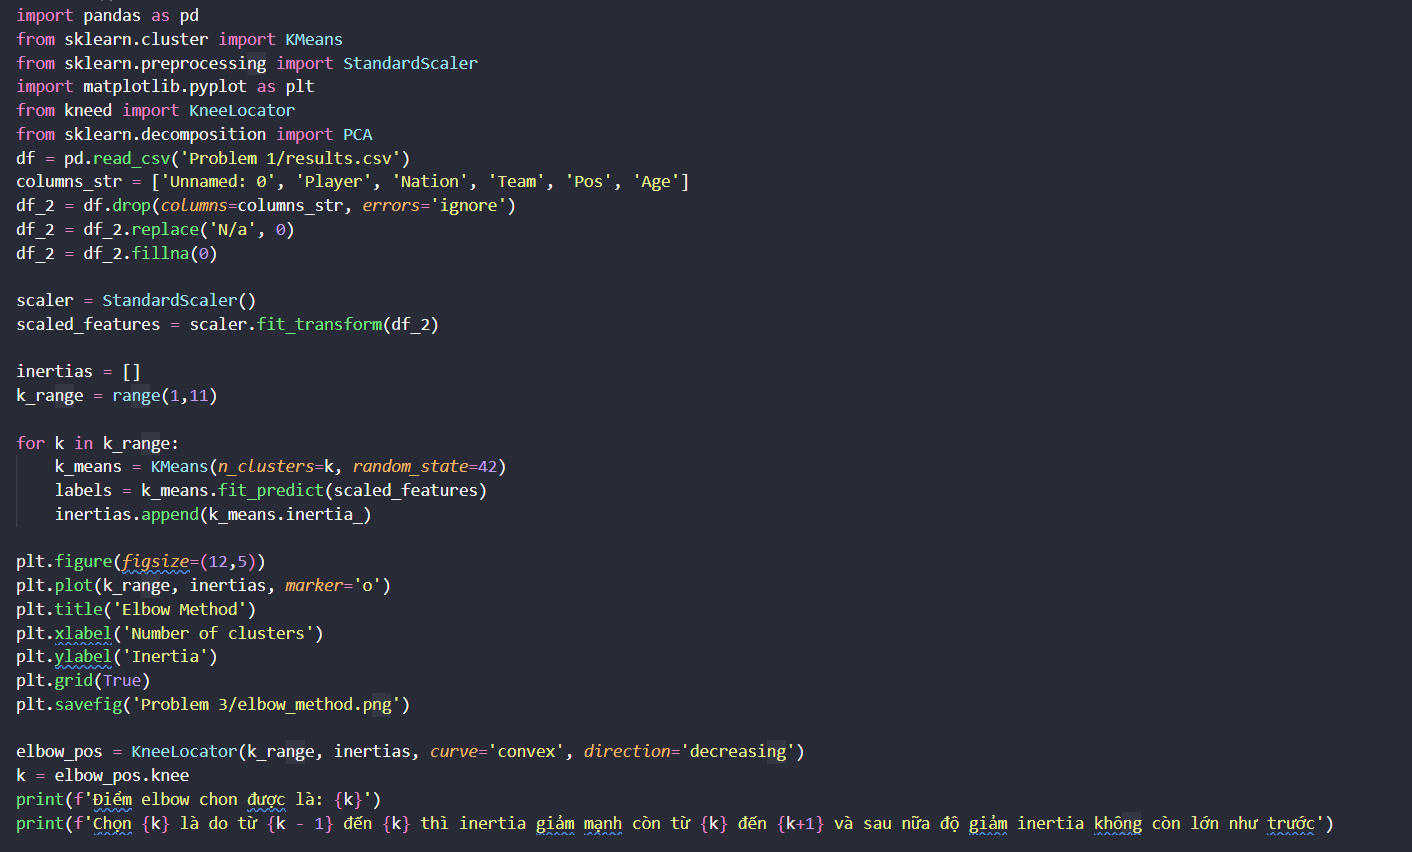
\includegraphics[width=1\linewidth]{img/3_1.png}
\end{figure}
- Đoạn code: 
\begin{verbatim}
columns_str = ['Unnamed: 0', 'Player', 'Nation', 'Team', 'Pos', 'Age']
df_2 = df.drop(columns=columns_str, errors='ignore')
df_2 = df_2.replace('N/a', 0)
df_2 = df_2.fillna(0)   
\end{verbatim}
Xứ lý dữ liệu gần giống câu 2 nhưng không trực tiếp lấy cột có dạng số mà loại bỏ các cột có dạng chữ. Thay tất cả 'N/a' và giá trị NaN sang giá trị 0.\\
- Chuẩn hóa dữ liệu để áp dụng các hàm sẵn có cho thuật toán k\_means:
\begin{verbatim}
    scaler = StandardScaler()
    scaled_features = scaler.fit_transform(df_2)
\end{verbatim}
- Khởi chạy đoạn code theo phương pháp elbow:
\begin{verbatim}
    inertias = []
    k_range = range(1,11)

    for k in k_range:
        k_means = KMeans(n_clusters=k, random_state=42)
        labels = k_means.fit_predict(scaled_features)
        inertias.append(k_means.inertia_)
\end{verbatim}
\begin{itemize}
    \item Khởi tạo danh sách \textbf{inertias}: Dùng để lưu trữ giá trị inertia cho mỗi số
    lượng cụm k.
    \item Lặp qua các giá trị \textbf{k} từ 1 đến 10 (với \textbf{range(1,11)}):
    \begin{itemize}[label=$\circ$]
        \item Đối với mỗi giá trị \textbf{k}, ta tạo một đối tượng \textbf{KMeans} và áp dụng phương thức \textbf{fit\_predict} để phân cụm dữ liệu.
        \item \textbf{fit\_predict} sẽ trả về labels (nhãn cụm cho từng điểm dữ liệu) và cập nhật đối tượng \textbf{k\_means}.
    \end{itemize}
    \item Lưu giá trị inertia vào danh sách \textbf{inertias}: Inertia là tổng bình phương khoảng cách từ các điểm đến tâm của cụm gần nhất, được tính qua \textbf{ k\_means.inertia\_}.
\end{itemize}
- Tiếp theo thực hiện vẽ biểu đồ Elbow method với trục x là số nhóm còn y là Inertia, có thể dựa vào biểu đồ tìm elbow hoặc có thể dùng thư viện knee để chính xác nhất:
\begin{verbatim}
    plt.figure(figsize=(12,5))
    plt.plot(k_range, inertias, marker='o')
    plt.title('Elbow Method')
    plt.xlabel('Number of clusters')
    plt.ylabel('Inertia')
    plt.grid(True)
    plt.savefig('Problem 3/elbow_method.png')
    
    elbow_pos = KneeLocator(k_range, inertias, curve='convex',direction=
    'decreasing')
    k = elbow_pos.knee
    print(f'Điểm elbow chon được là: {k}')
\end{verbatim}
\begin{figure}[H]
    \centering
    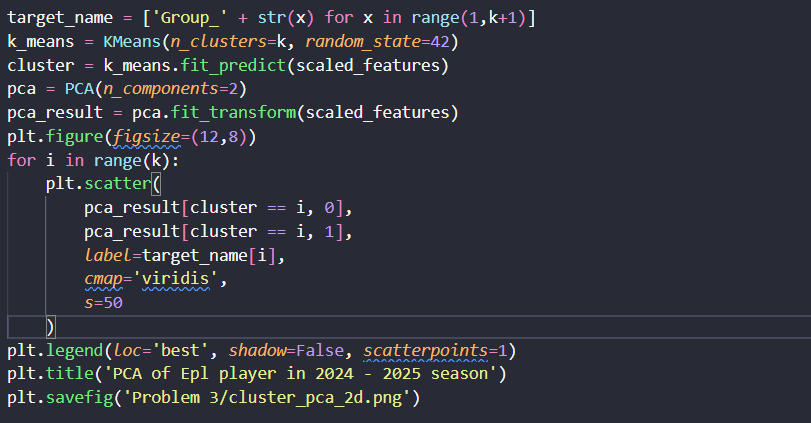
\includegraphics[width=1\linewidth]{img/3-2.png}
\end{figure}
- Tạo tên nhóm cụm (\textbf{target\_name}):
\begin{itemize}
    \item Tạo một danh sách tên nhóm có dạng ['Group\_1', 'Group\_2', ..., 'Group\_k'], với k là số cụm.
\end{itemize}
- Áp dụng \textbf{KMeans}:
\begin{itemize}
    \item \textbf{k\_means = KMeans(n\_clusters=k, random\_state=42)}: Khởi tạo đối tượng KMeans với số cụm \textbf{k}.
    \item \textbf{cluster = k\_means.fit\_predict(scaled\_features)}: Dự đoán nhóm cho các mẫu trong \textbf{scaled\_features} và lưu kết quả vào cluster.
\end{itemize}
- Áp dụng PCA:
\begin{itemize}
    \item \textbf{pca = PCA(n\_components=2)}: Khởi tạo đối tượng PCA để giảm chiều dữ liệu xuống 2 chiều.
    \item \textbf{pca\_result = pca.fit\_transform(scaled\_features)}: Áp dụng PCA lên dữ liệu chuẩn hóa \textbf{scaled\_features}.
\end{itemize}
- Vẽ biểu đồ phân cụm:
\begin{itemize}
    \item \textbf{plt.scatter()}: Vẽ các điểm trên biểu đồ 2D với màu sắc khác nhau cho từng nhóm cụm (cluster == i).
    \item \textbf{label=target\_name[i]}: Đặt tên cho mỗi nhóm tương ứng với các cụm.
    \item \textbf{plt.legend()}: Thêm chú thích vào biểu đồ.
    \item \textbf{plt.savefig()}: Lưu biểu đồ vào tệp \textbf{cluster\_pca\_2d.png}.
\end{itemize}

\cleardoublepage
\section{PHÂN TÍCH CÂU 4}
\addcontentsline{toc}{section}{\numberline {} PHÂN TÍCH CÂU 4}
\setcounter{section}{4}
* \textbf{Truy cập link github để có thể xem code tốt nhất:}  \url{https://github.com/DoTienThanh325/Big_exercise/tree/main/Problem%204}
\subsection{Câu 4 ý 1}
\subsubsection{Ý tưởng làm bài}
Sử dụng selenium để lấy dữ liệu của trang web, chuẩn hóa tên thu được sao cho dữ liệu tên mới thu được khớp với tên cầu thủ trong từ bài một thu được để đối chiếu thời gian thi đấu cầu thủ.
\subsubsection{Phân tích code câu 4 ý 1}
\begin{figure}[H]
    \centering
    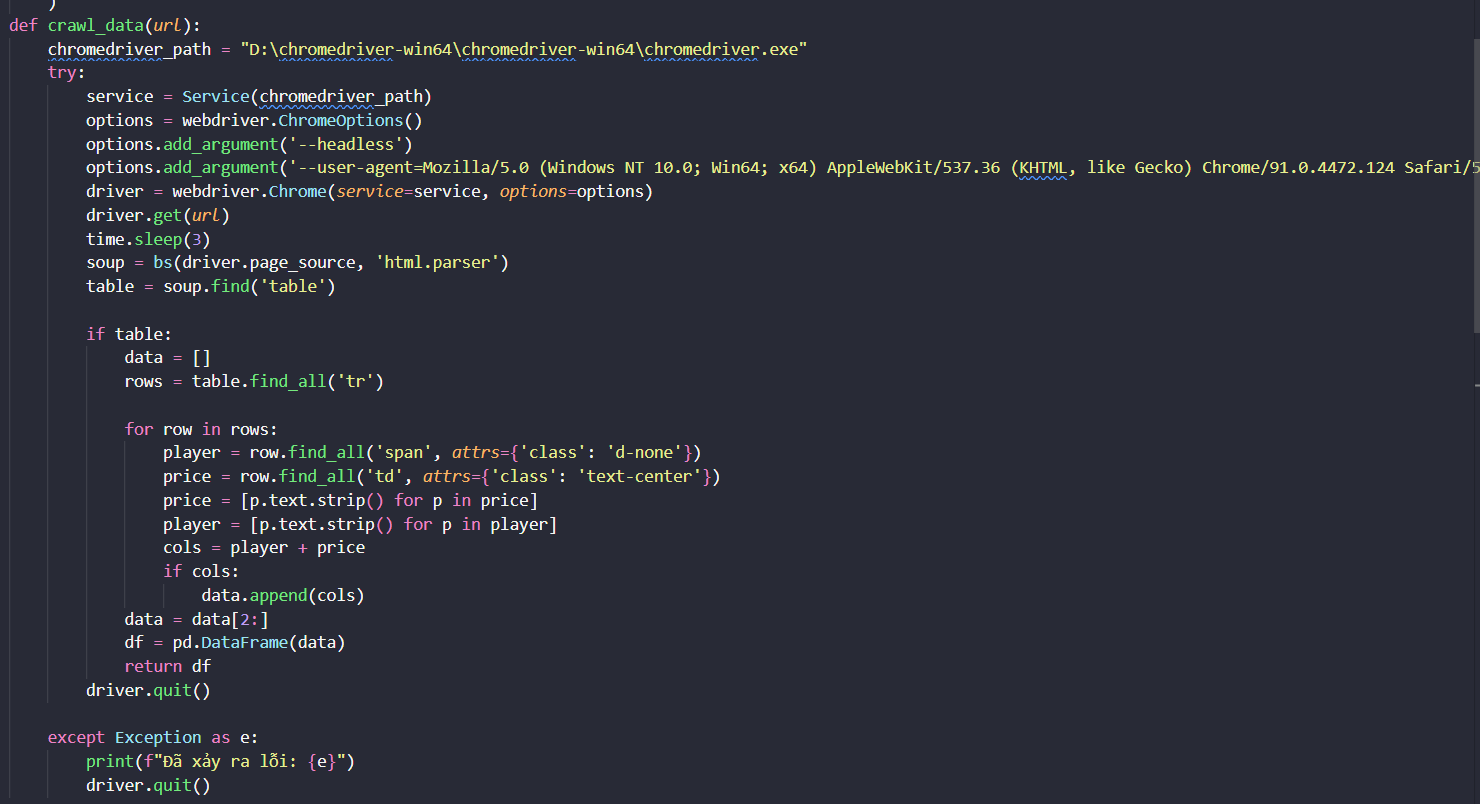
\includegraphics[width=1\linewidth]{img/4_1-1.png}
\end{figure}
- Hàm \textbf{crawl\_data()} Áp dụng Selenium:
\begin{itemize}
    \item \textbf{chromedriver\_path }: Khởi tạo biến đường dẫn chromedriver.
    \item \textbf{service = Service(chromedriver\_path)}: Khởi tạo một đối tượng Service để chỉ định đường dẫn đến trình điều khiển chromedriver (tệp cần thiết để Selenium tương tác với trình duyệt Chrome).
    \item \textbf{webdriver.ChromeOptions()}: Tạo một đối tượng \textbf{ChromeOptions} để thiết lập các tùy chọn cho Chrome.
    \begin{itemize}[label=$\circ$]
        \item \textbf{--headless}: Chạy Chrome mà không mở giao diện người dùng (trình duyệt sẽ chạy ở chế độ ẩn).
        \item \textbf{ --user-agent=Mozilla/...}: Thiết lập User-Agent để giả lập trình duyệt Chrome, tránh bị phát hiện là bot.
    \end{itemize}
    \item \textbf{driver = webdriver.Chrome(service=service, options=options)}: Khởi tạo trình duyệt Chrome với các tùy chọn đã thiết lập (bao gồm chế độ headless và user-agent).
    \item \textbf{driver.get(url)}: Truy cập vào URL.
    \item \textbf{time.sleep(3)}: Đợi 3 giây để trang web tải xong trước khi thu thập dữ liệu.
    \item \textbf{soup = bs(driver.page\_source, 'html.parser')}: Lấy nội dung trang web (HTML) và phân tích nó bằng BeautifulSoup.
    \item \textbf{table = soup.find('table')}: Tìm thẻ <table> đầu tiên trong nội dung trang.
    \item \textbf{if table}:: Kiểm tra nếu bảng dữ liệu tồn tại trên trang.
    \item \textbf{rows = table.find\_all('tr')}: Tìm tất cả các thẻ <tr> trong bảng, mỗi thẻ tương ứng với một hàng trong bảng.
    \item Lấy dữ liệu cầu thủ và giá chuyển nhượng:
    \begin{itemize}[label=$\circ$]
        \item \textbf{player = row.find\_all('span', attrs={'class': 'd-none'})}: Lấy các phần tử \textbf{<span>} có class \textbf{'d-none'}.
        \item \textbf{price = row.find\_all('td', attrs={'class': 'text-center'})}: Lấy các thẻ \textbf{<td>} có class \textbf{'text-center'}.
    \end{itemize}
    \item \textbf{price = [p.text.strip() for p in price]} và \textbf{player = [p.text.strip() for p in player]}: Loại bỏ khoảng trắng thừa từ các giá trị lấy được.
    \item \textbf{cols = player + price}: Kết hợp thông tin người chơi và giá vào một danh sách cols
    \item \textbf{if cols:}: Kiểm tra nếu danh sách cols không rỗng trước khi thêm vào data.
    \item \textbf{df = pd.DataFrame(data)}: Chuyển danh sách data thành một DataFrame của pandas.
    \item Sử dụng \textbf{try} và \textbf{except} để phòng trường hợp bị lỗi.
\end{itemize}
- Hàm chuẩn hóa tên cầu thủ: Do lấy dữ liệu từ hai trang web khác nhau nên tên cầu thủ không được giống nhau nên ta cần chuẩn hóa để cầu thủ hai nguồn dữ liệu khớp nhau:
\begin{figure}[H]
    \centering
    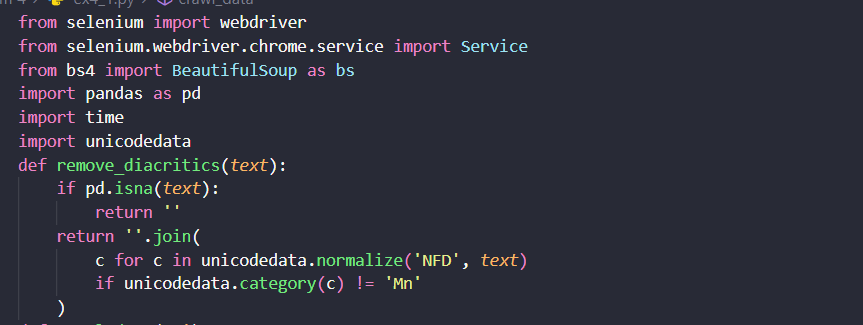
\includegraphics[width=1\linewidth]{img/4-1_2.png}
\end{figure}
- \textbf{if pd.isna(text): return ''}: Kiểm tra nếu đầu vào là giá trị NaN của pandas, trả về một chuỗi rỗng. Điều này giúp tránh lỗi khi hàm nhận giá trị NaN.\\
- \textbf{unicodedata.normalize('NFD', text)}: Sử dụng thư viện \textbf{unicodedata} của Python để chuẩn hóa chuỗi văn bản theo dạng "NFD" (Normalization Form Decomposed). Trong NFD, các ký tự có dấu được tách thành hai phần: ký tự cơ bản và dấu phụ. Ví dụ, chữ "é" sẽ được tách thành "e" và dấu sắc.\\
- \textbf{unicodedata.category(c) != 'Mn'}: Kiểm tra xem ký tự \textbf{c} có phải là dấu phụ hay không. \textbf{Mn} là mã phân loại cho các dấu phụ trong Unicode, và bạn loại bỏ các ký tự này trong quá trình ghép chuỗi.\\
- \textbf{''.join(c for c in ...)}: Kết hợp các ký tự lại thành một chuỗi mà không chứa dấu phụ.
\begin{figure}[H]
    \centering
    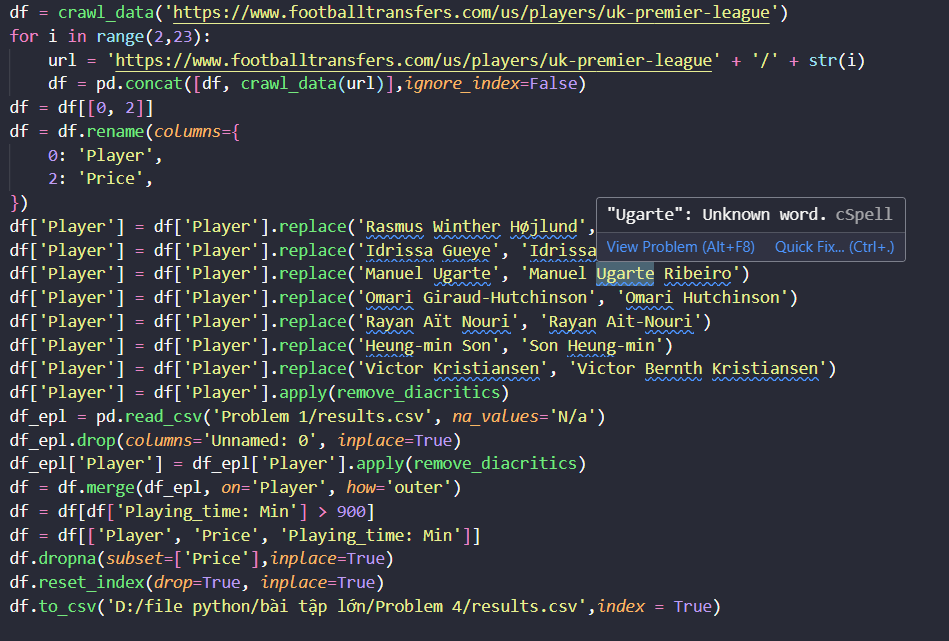
\includegraphics[width=1\linewidth]{img/4-1_3.png}
\end{figure}
- Chạy chương trình trong hàm main:
\begin{itemize}
    \item Lấy hết dữ liệu từ 22 url.
    \item \textbf{df = df[[0, 2]]}: Chỉ lấy hai cột chỉ số 0 và 2.
    \item \textbf{df = df.rename(columns={0: 'Player', 2: 'Price'})}: Đổi tên cột thành 'Player' và 'Price'.
    \item \textbf{df['Player'] = df['Player'].replace(...)}: Thực hiện thay thế tên một số cầu thủ đặc biệt sao khớp với dữ liệu câu 1.
    \item \textbf{df['Player'] = df['Player'].apply(remove\_diacritics)}: Áp dụng hàm \textbf{remove\_diacritics} để loại bỏ dấu phụ, chuẩn hóa tên.
    \item \textbf{df\_epl = pd.read\_csv('Problem 1/results.csv', na\_values='N/a')}: Đọc dữ liệu thu được từ câu 1.
    \item \textbf{df\_epl.drop(columns='Unnamed: 0', inplace=True)}: Xóa cột \textbf{'Unnamed: 0'} không cần thiết.
    \item \textbf{df\_epl['Player'] = df\_epl['Player'].apply(remove\_diacritics)}: Áp dụng hàm \textbf{remove\_diacritics} cho cột 'Player' của tệp CSV.
    \item \textbf{ df = df.merge(df\_epl, on='Player', how='outer')}: Kết hợp dữ liệu từ hai DataFrame (\textbf{df và df\_epl}) theo cột \textbf{'Player'}, dùng kiểu kết hợp \textbf{'outer'} để giữ tất cả các cầu thủ trong cả hai DataFrame.
    \item \textbf{df = df[df['Playing\_time: Min'] > 900]}: Lọc ra các cầu thủ có thời gian chơi hơn 900 phút.
    \item \textbf{df = df[['Player', 'Price', 'Playing\_time: Min']]}: Chọn chỉ các cột \textbf{'Player'}, \textbf{'Price'}, và \textbf{'Playing\_time: Min'}.
    \item \textbf{df.dropna(subset=['Price'], inplace=True)}: Loại bỏ các dòng có giá trị 'Price' là NaN.
    \item \textbf{df.reset\_index(drop=True, inplace=True)}: Đặt lại index của DataFrame.
    \item \textbf{df.to\_csv('D:/file python/bài tập lớn/Problem 4/results.csv', index=True)}: Lưu lại DataFrame hoàn chỉnh.
\end{itemize}
\subsection{Câu 4 ý 2}
\subsubsection{Ý tưởng làm bài}
Xử lý hai bảng giá trị đã có ở câu 4 ý 1 và câu 1 sao cho khớp dữ liệu sau đó huấn luyện mô hình theo mô hình LogisticRegression.
\subsubsection{Phân tích code câu 4 ý 2}
- \textbf{Bước 1:} Xứ lý dữ liệu cầu thủ và giá tiền:
\begin{figure}[H]
    \centering
    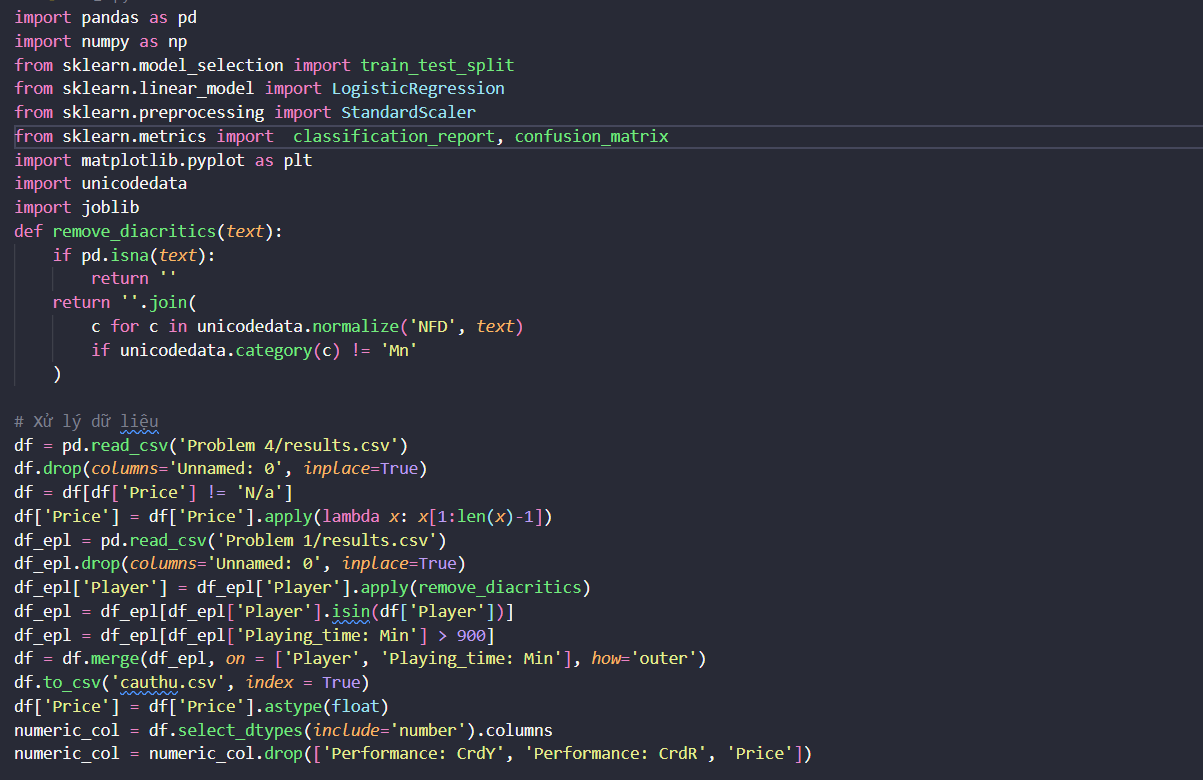
\includegraphics[width=1\linewidth]{img/4_2-1.png}
\end{figure}
- Đoạn code trên lấy dữ liệu từ hai file csv của câu 1 và ý 1 câu 4 xử lý lại tên sao cho khớp dữ liệu sau đó gộp các thuộc tính cầu thủ lại. Thu lấy các cột chỉ số có dạng number để phân tích dự đoán giá cầu thủ.
Loại bỏ các chỉ số như giá cầu thủ, thẻ đỏ, thẻ vàng vì không ảnh hưởng tới giá của cầu thủ.\\\\
- \textbf{Bước 2:} Huấn luyện mô hình:
\begin{figure}[H]
    \centering
    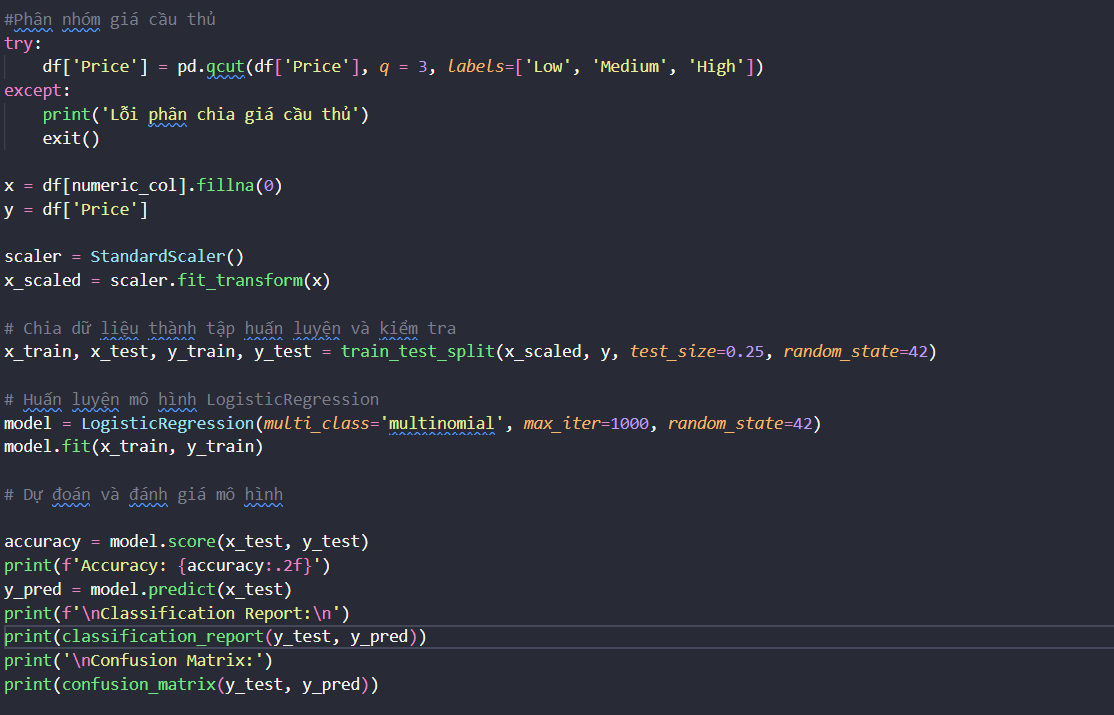
\includegraphics[width=1\linewidth]{img/4-2_2.png}
\end{figure}
- Phân nhóm giá trị Price thành 3 nhóm: \textbf{Low, Medium, High} bằng \textbf{qcut}.\\
- Chuẩn hóa các cột số \textbf{numeric\_col} bằng \textbf{StandardScaler}.\\
- Chia dữ liệu thành tập huấn luyện và kiểm tra.
- Huấn luyện mô hình \textbf{LogisticRegression} đa lớp (\textbf{multi\_class='multinomial'}) để dự đoán nhóm giá.
- Đánh giá độ chính xác (\textbf{accuracy}), báo cáo phân loại (\textbf{classification\_report}), và ma trận nhầm lẫn (\textbf{confusion\_matrix}).\\\\
- \textbf{Bước 3:} Thu lấy dataframe tầm quan trọng thuộc tính:
\begin{figure}[H]
    \centering
    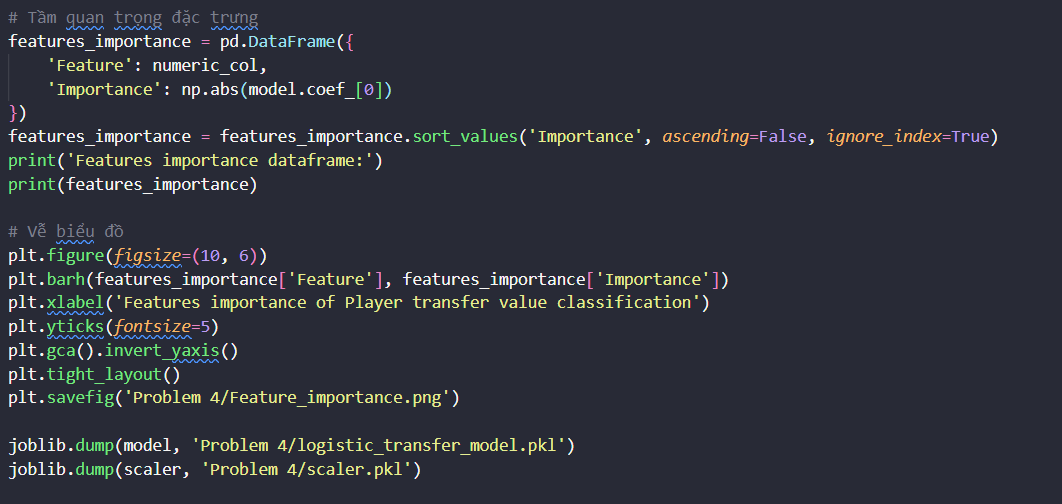
\includegraphics[width=1\linewidth]{img/4_2-3.png}
\end{figure}
- Tạo dataframe để lưu thuộc tính và tầm quan trọng của nó.\\
- Sắp xếp các giá trị theo thứ tự giảm dần.\\
- In ra và vẽ dưới dạng biểu đồ.
- Cuối cùng lưu mô hình vào file.
\end{document}  